\chapter{Photosynthesis}\label{ch:g12:photosynthesis}

Put a sprig of pondweed upside down in a jar of water under a lamp,
and a stream of bubbles rises from the cut stem: oxygen, one bubble
every few seconds, faster if the lamp is brought closer, stopping when
it is switched off. The gas is the visible half of a process that is
feeding every animal on the planet and that made the air breathable
two billion years ago. \cref{ch:g10:cell-metabolism} gave it in one
line: carbon dioxide and water, with light, become sugar and oxygen.
This chapter opens the \omterm{def:g12:photosynthesis:chloroplast}{chloroplast} and follows the energy of a photon
into a chemical bond.

\section{The chloroplast}

\begin{definition}[Chloroplast]\label{def:g12:photosynthesis:chloroplast}
The \emph{chloroplast}\index{chloroplast} is the \omterm{def:g10:cells-common-unit:organelle}{organelle} of
\omterm{def:g10:cell-metabolism:autotrophy}{photosynthesis}: a lens-shaped body some \qty{5}{\micro m} long, bounded
by a double membrane, containing a fluid, the \emph{stroma}, in which
lie stacks of flattened membrane sacs, the \emph{thylakoids}\index{thylakoid}.
The thylakoid membranes hold the pigments --- \emph{chlorophylls} a
and b, green, and orange carotenoids --- and the \omterm{def:g11:gene-expression:protein}{proteins} that convert
light energy; the stroma holds the \omterm{def:g11:enzymes-and-phenotype:enzyme}{enzymes} that build sugar. A leaf
\omterm{def:g10:cells-common-unit:cell}{cell} contains tens of \omterm{def:g10:cells-common-unit:organelle}{chloroplasts}, a square millimetre of leaf some
half a million.
\end{definition}

\begin{omfigure}
\begin{tikzpicture}
  \node[anchor=south west, inner sep=0] (img) at (0,0)
    {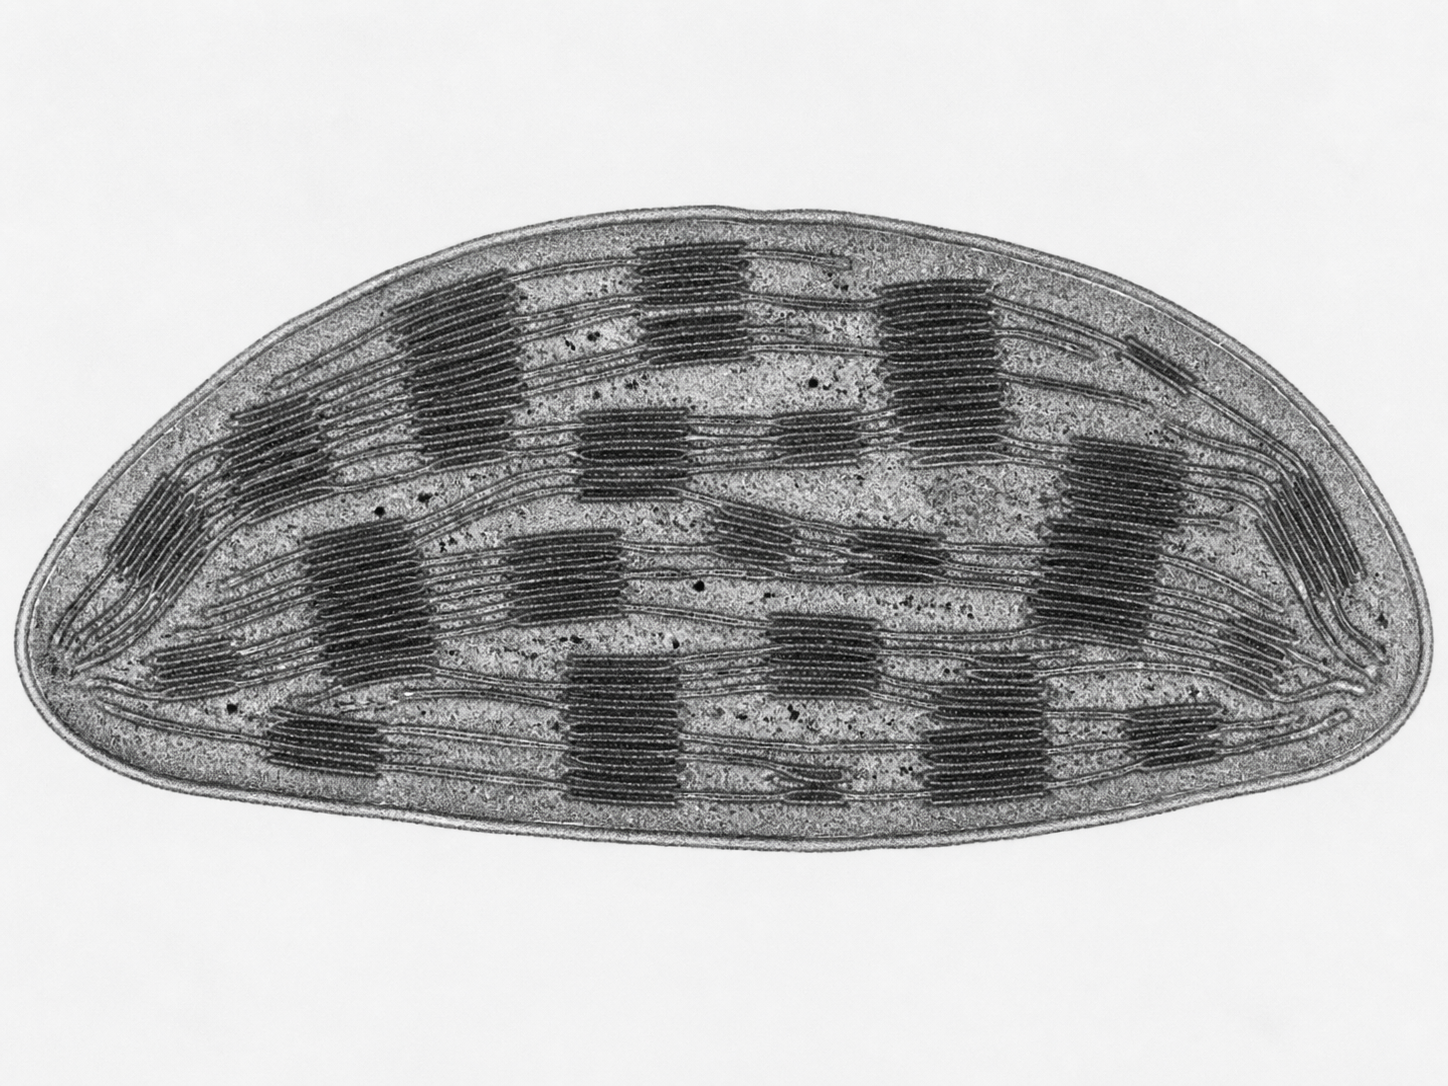
\includegraphics[width=0.5\linewidth]{images/book2/ai/g12-photo-chloroplast-tem.png}};
  \begin{scope}[x={(img.south east)}, y={(img.north west)},
      every node/.style={font=\small}]
    \draw[omDef, thick] (0.10,0.50) -- (-0.04,0.80) node[left, align=right] {double\\ envelope};
    \draw[omDef, thick] (0.47,0.72) -- (0.47,1.06) node[above] {stacked thylakoids (a granum)};
    \draw[omDef, thick] (0.62,0.42) -- (1.04,0.20) node[right] {stroma};
    \draw[omDef, thick] (0.80,0.60) -- (1.04,0.75) node[right, align=left] {membranes joining\\ the stacks};
  \end{scope}
\end{tikzpicture}

{\small A \omterm{def:g12:photosynthesis:chloroplast}{chloroplast} in the electron microscope: the double envelope,
the stroma, and the \omterm{def:g12:photosynthesis:chloroplast}{thylakoid} membranes stacked into grana, where the
pigments sit. Light is captured in the membranes; sugar is built in the
fluid around them.}
\end{omfigure}

\begin{proposition}[Which light is used]\label{prop:g12:photosynthesis:spectrum}
Chlorophyll absorbs blue and red light strongly and green light
hardly at all --- which is why leaves are green. \omterm{def:g10:cell-metabolism:autotrophy}{Photosynthesis} is
driven by the wavelengths the pigments absorb: measured against
wavelength, its rate (the \emph{action spectrum}) rises and falls with
the pigments' absorption, with peaks in the blue and the red and a
trough in the green.
\end{proposition}
\begin{proof}[Evidence]
Engelmann (1882) laid a filament of green alga in a drop of water
containing bacteria that swim towards oxygen, and projected a spectrum
along the filament through the microscope: the bacteria gathered
around the segments lit in blue and in red, and avoided the green ---
oxygen was being released where those colours fell. Modern
measurement of oxygen output under coloured lamps gives the same
curve, and it matches the absorption spectrum of the extracted
pigments.
\end{proof}

\begin{omfigure}
\begin{tikzpicture}
\begin{axis}[
  width=0.88\linewidth, height=5.8cm,
  axis x line=bottom, axis y line=left,
  xmin=400, xmax=700, ymin=0, ymax=110,
  xlabel={wavelength (nm)}, ylabel={\% of maximum},
  xlabel style={font=\small, at={(axis description cs:0.5,-0.12)}, anchor=north},
  ylabel style={font=\small},
  tick label style={font=\small}, xtick={400,450,500,550,600,650,700}, ytick={0,50,100},
  legend style={at={(0.5,-0.3)}, anchor=north, legend columns=2, font=\small, draw=none},
]
\addplot[thick, omMeth, smooth] coordinates {(400,70) (430,100) (450,75) (480,35) (500,15) (550,8) (600,15) (640,45) (665,90) (680,70) (700,10)};
\addplot[thick, omThm, dashed, smooth] coordinates {(400,65) (430,85) (450,80) (480,55) (500,35) (550,25) (600,35) (640,60) (665,95) (680,100) (700,20)};
\legend{absorption by leaf pigments, rate of photosynthesis (action spectrum)}
\end{axis}
\end{tikzpicture}

{\small Absorption of light by the extracted pigments of a leaf, and
the rate of \omterm{def:g10:cell-metabolism:autotrophy}{photosynthesis} of the leaf, against wavelength. Both peak
in the blue and the red and dip in the green: the light that drives
\omterm{def:g10:cell-metabolism:autotrophy}{photosynthesis} is the light the pigments absorb.}
\end{omfigure}

\section{The light phase: water split, energy stored}

\begin{proposition}[What happens in the thylakoids]\label{prop:g12:photosynthesis:lightphase}
In the \omterm{def:g12:photosynthesis:chloroplast}{thylakoid} membranes, in the light, three things happen
together:
\begin{itemize}
  \item water molecules are \emph{split}: their oxygen is released as
        $\mathrm{O_2}$ --- the oxygen of \omterm{def:g10:cell-metabolism:autotrophy}{photosynthesis} comes from
        water, not from carbon dioxide --- and their hydrogen is
        retained as electrons and protons;
  \item the energy of the absorbed photons is used to load those
        electrons onto a carrier molecule, \emph{reduced NADP}, which
        the stroma will use as a source of hydrogen;
  \item the same energy drives the synthesis of \emph{ATP}.
\end{itemize}
The light phase thus converts light into two chemical products, ATP
and reduced NADP, and releases oxygen as a by-product. No carbon
dioxide is involved.
\end{proposition}
\begin{proof}[Evidence]
Hill (1937) illuminated isolated \omterm{def:g10:cells-common-unit:organelle}{chloroplasts} in water with an
artificial electron acceptor and no carbon dioxide: they released
oxygen and reduced the acceptor. So oxygen release needs light and
water but not $\mathrm{CO_2}$, and is coupled to the transfer of
electrons. Ruben and Kamen (1941) supplied algae with water containing
the heavy isotope $^{18}$O: the oxygen released was heavy; supplied
with heavy carbon dioxide and ordinary water, it was not. The oxygen
comes from the water.
\end{proof}

\begin{omfigure}
\begin{tikzpicture}[font=\small, >=Stealth,
  b/.style={draw, rounded corners, align=center, minimum height=1.0cm}]
  % thylakoid box
  \node[b, fill=omMeth!15, text width=3.6cm, minimum height=3.2cm] (thy) at (0,0) {};
  \node[anchor=north, font=\small\bfseries] at (thy.north) {thylakoid membranes};
  \node[font=\small, align=center] at (0,-0.1) {light absorbed\\ by chlorophyll};
  % stroma box
  \node[b, fill=omDef!10, text width=3.6cm, minimum height=3.2cm] (str) at (6.4,0) {};
  \node[anchor=north, font=\small\bfseries] at (str.north) {stroma};
  \node[font=\small, align=center] at (6.4,-0.1) {Calvin cycle:\\ $\mathrm{CO_2}$ fixed\\ into sugar};
  % inputs/outputs
  \draw[->, thick, omProp] (-3.2,1.0) -- (thy.west |- 0,1.0) node[pos=0, left, omProp] {light};
  \draw[->, thick] (-3.2,-0.6) -- (thy.west |- 0,-0.6) node[pos=0, left] {$\mathrm{H_2O}$};
  \draw[->, thick] (thy.south) -- ++(0,-1.0) node[below] {$\mathrm{O_2}$ released};
  \draw[->, thick, omThm] (thy.east |- 0,0.7) -- (str.west |- 0,0.7) node[midway, above] {ATP};
  \draw[->, thick, omThm] (thy.east |- 0,-0.3) -- (str.west |- 0,-0.3) node[midway, above] {reduced NADP};
  \draw[->, thick, gray] (str.west |- 0,-1.1) -- (thy.east |- 0,-1.1) node[midway, below, font=\scriptsize] {carriers return};
  \draw[->, thick] (9.6,0.6) -- (str.east |- 0,0.6) node[pos=0, right] {$\mathrm{CO_2}$};
  \draw[->, thick] (str.east |- 0,-0.6) -- (9.6,-0.6) node[right] {sugar};
\end{tikzpicture}

{\small The two phases of \omterm{def:g10:cell-metabolism:autotrophy}{photosynthesis}. In the \omterm{def:g12:photosynthesis:chloroplast}{thylakoid} membranes,
light splits water, releases oxygen and charges two carriers, ATP and
reduced NADP. In the stroma those carriers pay for the fixation of
carbon dioxide into sugar. The first phase needs light; the second
needs only its products.}
\end{omfigure}

\section{The carbon phase: sugar built}

\begin{proposition}[The Calvin cycle]\label{prop:g12:photosynthesis:calvin}
In the stroma, carbon dioxide is attached, one molecule at a time, to
a five-carbon sugar already present, by the most abundant \omterm{def:g11:enzymes-and-phenotype:enzyme}{enzyme} on
Earth; the six-carbon product splits at once into two three-carbon
molecules, which are reduced --- using the ATP and the reduced NADP of
the light phase --- into three-carbon sugars. Most of these are
recycled to regenerate the five-carbon acceptor, closing the
\emph{Calvin cycle}\index{Calvin cycle}; one in six leaves the cycle
as the plant's net gain. Three turns of the cycle, three
$\mathrm{CO_2}$ fixed, nine ATP and six reduced NADP spent: one
three-carbon sugar exported. Two of them make a glucose.
\end{proposition}
\begin{proof}[Evidence]
Calvin (1950s) gave algae carbon dioxide labelled with radioactive
$^{14}$C for a few seconds, killed them in boiling alcohol, and
separated their molecules: after five seconds the label was in a
single three-carbon acid; after thirty, in three-carbon sugars and the
five-carbon acceptor; after minutes, in sucrose and starch. Cutting
off the light left the acceptor unregenerated and the three-carbon
acid accumulating; cutting off the $\mathrm{CO_2}$ left the acceptor
accumulating. The order of appearance is the order of the cycle.
\end{proof}

\begin{omfigure}
\begin{tikzpicture}[font=\small, >=Stealth]
  \draw[thick, ->] (90:2.2) arc (90:-30:2.2);
  \draw[thick, ->] (-30:2.2) arc (-30:-150:2.2);
  \draw[thick, ->] (-150:2.2) arc (-150:-270:2.2);
  \node[draw, rounded corners, fill=omDef!12, align=center, font=\small] at (90:2.2) {5-carbon\\ acceptor ($\times 3$)};
  \node[draw, rounded corners, fill=omProp!15, align=center, font=\small] at (-30:2.2) {3-carbon acid\\ ($\times 6$)};
  \node[draw, rounded corners, fill=omMeth!15, align=center, font=\small] at (-150:2.2) {3-carbon sugar\\ ($\times 6$)};
  \draw[->, thick] (3.6,2.2) -- (2.4,1.6) node[pos=0, right, align=left] {$3\,\mathrm{CO_2}$ enter};
  \draw[->, thick, omThm] (2.2,-2.4) -- (1.2,-2.0) node[pos=0, right, omThm, align=left] {6 ATP, 6 reduced NADP\\ from the light phase};
  \draw[->, thick, omThm] (-3.6,1.0) -- (-2.2,1.4) node[pos=0, left, omThm] {3 ATP};
  \draw[->, thick] (-2.4,-2.4) -- (-3.6,-3.2) node[anchor=north, align=center] {1 three-carbon sugar leaves:\\ half a glucose};
  \node[font=\scriptsize, align=center] at (0,0) {5 of the 6 sugars\\ rebuild the\\ 3 acceptors};
\end{tikzpicture}

{\small The \omterm{prop:g12:photosynthesis:calvin}{Calvin cycle}, counted for three turns. Three carbon
dioxides join three five-carbon acceptors; the six three-carbon
products are reduced to sugars at the cost of the light phase's ATP
and reduced NADP; five of the six are recycled into the acceptors and
one is the gain.}
\end{omfigure}

\begin{example}[The bookkeeping of a glucose]\label{ex:g12:photosynthesis:bookkeeping}
One glucose needs six carbon dioxides, hence six turns of the cycle,
18 ATP and 12 reduced NADP, all supplied by the light phase, which
splits 12 water molecules and releases six oxygens to make them. Net:
$6\,\mathrm{CO_2} + 12\,\mathrm{H_2O} \to \mathrm{C_6H_{12}O_6} +
6\,\mathrm{O_2} + 6\,\mathrm{H_2O}$ --- the summary equation of
\cref{ch:g10:cell-metabolism}, now with the water on both sides,
since the oxygen released comes from the water split, not from the
carbon dioxide.
\end{example}

\begin{omfigure}
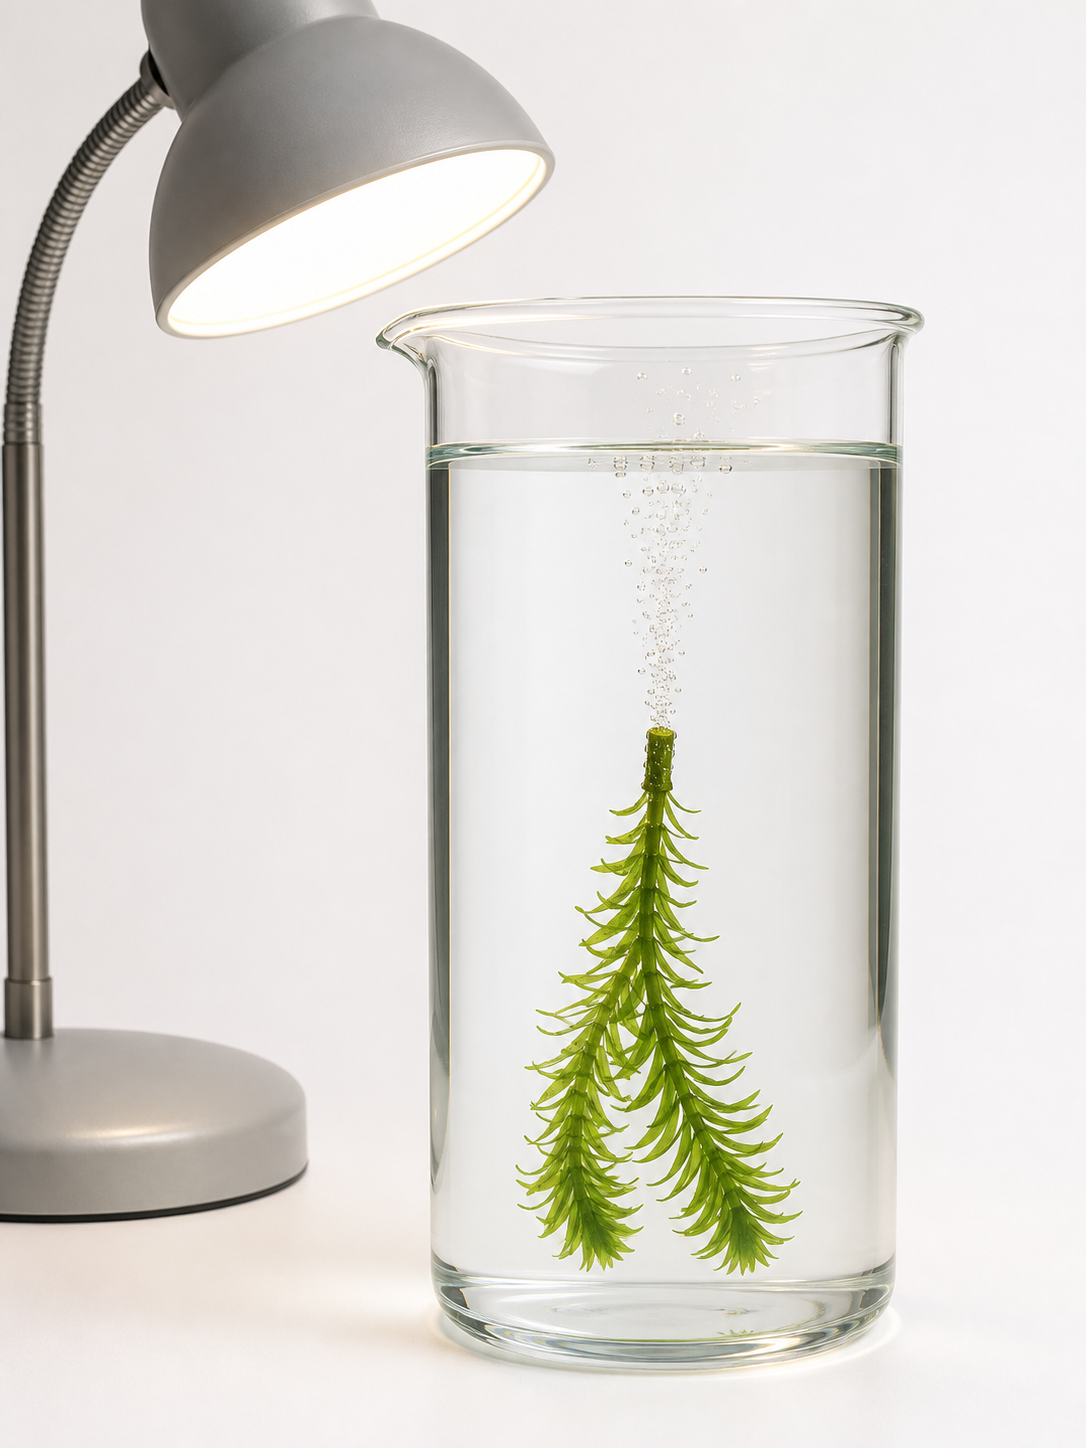
\includegraphics[width=0.34\linewidth]{images/book2/ai/g12-photo-elodea-bubbles.png}

{\small Pondweed under a lamp: the bubbles rising from the cut stem are
the oxygen of the light phase. Count them per minute, move the lamp,
change its colour, and the rate of \omterm{def:g10:cell-metabolism:autotrophy}{photosynthesis} is measured.}
\end{omfigure}

\section{What the sugar becomes, and how much there is}

\begin{proposition}[Fates of the product]\label{prop:g12:photosynthesis:fates}
The three-carbon sugars leaving the cycle are assembled, in the
\omterm{def:g12:photosynthesis:chloroplast}{chloroplast}, into \emph{starch}, the leaf's daytime store, or exported
to the \omterm{def:g10:cells-common-unit:cell}{cytoplasm} and turned into \emph{sucrose}, the sugar the \omterm{prop:g12:plant-rooted-life:saps}{phloem}
carries (\cref{ch:g12:plant-rooted-life}). From these the plant makes
everything else: cellulose for walls, \omterm{def:g10:chemistry-of-life:families}{lipids}, and --- with nitrogen and
sulfur from the soil --- \omterm{def:g10:chemistry-of-life:families}{amino acids} and \omterm{def:g10:universal-dna:nucleotide}{nucleotides}. \omterm{def:g10:cell-metabolism:autotrophy}{Photosynthesis}
is the source not only of the plant's energy but of all its \omterm{def:g10:chemistry-of-life:mineral-organic}{organic
matter}, and, through the food chains, of almost all \omterm{def:g10:chemistry-of-life:mineral-organic}{organic matter} on
Earth.
\end{proposition}
\admitted

\begin{example}[Efficiency, from leaf to planet]\label{ex:g12:photosynthesis:efficiency}
Full sunlight delivers about \qty{1000}{W} per square metre, of which
about 45\% is in wavelengths the pigments can use; a leaf converts at
best some 5\% of that into sugar during the day, and a crop, over a
season, 1\% to 2\% of the total sunlight into biomass. Small as the
fraction is, the sum is immense: \omterm{def:g10:cell-metabolism:autotrophy}{photosynthesis} fixes about
\qty{1e11}{t} of carbon a year --- a seventh of the carbon in the
atmosphere --- and releases the oxygen that respiration, fire and
rust consume.
\end{example}

\begin{method}[Reasoning about a photosynthesis experiment]\label{met:g12:photosynthesis:experiment}
\begin{enumerate}
  \item Identify what is measured: oxygen released (the light phase),
        carbon dioxide taken up or sugar formed (the carbon phase), or
        biomass (everything, over time).
  \item Identify what is varied: light (intensity, colour), carbon
        dioxide, temperature, water --- and which phase it acts on.
  \item Remember that the plant respires at the same time: a
        measured oxygen output is production minus respiration; in the
        dark only respiration shows (\cref{ch:g10:cell-metabolism}).
  \item Trace labels: $^{18}$O in water appears in the oxygen; $^{14}$C
        in carbon dioxide appears in the sugars, in the order of the
        cycle.
\end{enumerate}
\end{method}

\begin{remark}[Light, and then chemistry]\label{rem:g12:photosynthesis:light}
The only step of \omterm{def:g10:cell-metabolism:autotrophy}{photosynthesis} that needs light is the first: the
loading of electrons from water onto a carrier, with the release of
oxygen. Everything after --- the making of ATP, the fixation of carbon
dioxide, the building of sugar --- is chemistry that continues in the
dark as long as the carriers last, and that the next chapter's
respiration will run in reverse. The \omterm{def:g12:photosynthesis:chloroplast}{chloroplast} is where sunlight is
turned into chemical currency; the rest of the \omterm{def:g10:cells-common-unit:cell}{cell}, and the rest of
the biosphere, spends it.
\end{remark}

\section{Exercises}

\begin{exercise}[$\star$]\label{exo:g12:photosynthesis:1}
Describe the \omterm{def:g12:photosynthesis:chloroplast}{chloroplast} and say where the pigments and where the
sugar-building \omterm{def:g11:enzymes-and-phenotype:enzyme}{enzymes} are.
\end{exercise}

\begin{exercise}[$\star$]\label{exo:g12:photosynthesis:2}
Why are leaves green? Which colours drive \omterm{def:g10:cell-metabolism:autotrophy}{photosynthesis} best?
\end{exercise}

\begin{exercise}[$\star$]\label{exo:g12:photosynthesis:3}
List the three products of the light phase and say which is a
by-product.
\end{exercise}

\begin{exercise}[$\star$]\label{exo:g12:photosynthesis:4}
Where does the oxygen released by a plant come from, and how was it
shown?
\end{exercise}

\begin{exercise}[$\star$]\label{exo:g12:photosynthesis:5}
How many carbon dioxide molecules, ATP and reduced NADP does one
glucose require?
\end{exercise}

\begin{exercise}[$\star\star$]\label{exo:g12:photosynthesis:6}
From the spectrum figure, read the absorption and the photosynthetic
rate at \qty{550}{nm} and at \qty{665}{nm}. A greenhouse is lit with
green lamps to save energy: comment.
\end{exercise}

\begin{exercise}[$\star\star$]\label{exo:g12:photosynthesis:7}
Interpret Engelmann's experiment step by step: what the bacteria
detect, why they gather where they do, and what the experiment
establishes.
\end{exercise}

\begin{exercise}[$\star\star$]\label{exo:g12:photosynthesis:8}
Isolated \omterm{def:g10:cells-common-unit:organelle}{chloroplasts} in water, in the light, with an artificial
electron acceptor and no $\mathrm{CO_2}$, release oxygen. What does
this show about the relation between oxygen release and carbon
fixation?
\end{exercise}

\begin{exercise}[$\star\star$]\label{exo:g12:photosynthesis:9}
In Calvin's experiment the light is switched off while $\mathrm{CO_2}$
continues: the three-carbon acid accumulates and the five-carbon
acceptor disappears. Explain both observations.
\end{exercise}

\begin{exercise}[$\star\star$]\label{exo:g12:photosynthesis:10}
A pondweed releases 30 bubbles per minute under a lamp at
\qty{20}{cm}; at \qty{40}{cm} it releases 8. Explain, and predict the
count in the dark.
\end{exercise}

\begin{exercise}[$\star\star$]\label{exo:g12:photosynthesis:11}
A leaf fixes \qty{8}{g} of $\mathrm{CO_2}$ per square metre per hour.
What mass of glucose is that, and what mass of oxygen is released?
(Molar masses: $\mathrm{CO_2}$ 44, glucose 180, $\mathrm{O_2}$ 32
\unit{g/mol}.)
\end{exercise}

\begin{exercise}[$\star\star\star$]\label{exo:g12:photosynthesis:12}
Explain why the carbon phase is often called the "dark phase" and why
the name is misleading, using what happens to it in a plant kept in
the dark for an hour.
\end{exercise}

\begin{exercise}[$\star\star\star$]\label{exo:g12:photosynthesis:13}
A plant given water labelled with $^{18}$O and carbon dioxide
labelled with $^{14}$C. Say where each label is found after a minute,
after an hour, and after a day.
\end{exercise}

\begin{exercise}[$\star\star\star$]\label{exo:g12:photosynthesis:14}
Full sun delivers \qty{1000}{W/m^2}. A leaf stores \qty{20}{W/m^2} of
it as sugar. Compute the efficiency; then list three places where the
rest goes.
\end{exercise}

\begin{exercise}[$\star\star\star$]\label{exo:g12:photosynthesis:15}
The oxygen of the atmosphere (21\%) is entirely of photosynthetic
origin. Explain why an Earth without \omterm{def:g10:cell-metabolism:autotrophy}{photosynthesis} would lose its
oxygen within some thousands of years, and what this says about the
first two billion years of the planet.
\end{exercise}

\section{Problem: A Square Metre of Leaf}

\begin{problem}[{Weekend problem --- the energy of sunlight followed
into sugar: photons counted, carriers reckoned, oxygen and carbon
balanced, and a leaf's efficiency computed}]
\label{pb:g12:photosynthesis:1}
A square metre of leaf in full sun receives \qty{1000}{W}, of which
\qty{450}{W} lie in the wavelengths the pigments absorb; it fixes
\qty{8}{g} of $\mathrm{CO_2}$ per hour. Glucose holds \qty{2870}{kJ}
per mole. Molar masses: $\mathrm{CO_2}$ 44, $\mathrm{O_2}$ 32,
$\mathrm{H_2O}$ 18, glucose \qty{180}{g/mol}.

\medskip
\noindent\textbf{Part I --- Carbon and oxygen.}
\begin{enumerate}
  \item How many moles of $\mathrm{CO_2}$ does the leaf fix per hour?
  \item How many moles, and grams, of glucose does that make?
  \item How many moles of $\mathrm{O_2}$ are released, and what volume
        is that (\qty{24}{L} per mole)?
  \item How many water molecules are split to release that oxygen?
        How does this compare with the \qty{600}{mL} of water the
        square metre transpires in the hour?
  \item Where does each oxygen atom of the released $\mathrm{O_2}$ come
        from, and how do you know?
\end{enumerate}

\medskip
\noindent\textbf{Part II --- The carriers.}
\begin{enumerate}[resume]
  \item How many turns of the \omterm{prop:g12:photosynthesis:calvin}{Calvin cycle} are needed per hour?
  \item How many ATP and how many reduced NADP does the light phase
        supply per hour?
  \item Each reduced NADP carries two electrons taken from water. How
        many water molecules must be split per hour to supply them?
        Compare with question 4.
  \item If the leaf's light phase stopped (say, the \omterm{def:g10:cells-common-unit:organelle}{chloroplasts} were
        poisoned for water splitting), which of ATP, reduced NADP,
        oxygen and sugar would stop being made, and in what order?
  \item If instead the $\mathrm{CO_2}$ were removed, what would happen
        to the light phase within seconds, and why?
\end{enumerate}

\medskip
\noindent\textbf{Part III --- Energy.}
\begin{enumerate}[resume]
  \item Compute the energy stored in the glucose made per hour, in
        kilojoules, then as a power in watts.
  \item Compute the leaf's efficiency relative to the full sunlight,
        and relative to the absorbed wavelengths.
  \item A photon of red light (\qty{680}{nm}) carries about
        \qty{176}{kJ} per mole of photons. Fixing one $\mathrm{CO_2}$
        needs about 8 photons. Compute the energy of the photons used
        per mole of $\mathrm{CO_2}$ and compare with the energy stored
        per mole of $\mathrm{CO_2}$ fixed ($2870/6$).
  \item What fraction of the energy of the absorbed photons ends in the
        glucose? Where does the rest go?
  \item The leaf also respires \qty{0.5}{g} of glucose per hour. What
        is its net gain, and how would you measure it?
\end{enumerate}

\medskip
\noindent\textbf{Part IV --- From the leaf to the planet.}
Plants fix about \qty{1e11}{t} of carbon a year; the atmosphere holds
about \qty{8.5e11}{t} of carbon as $\mathrm{CO_2}$; the ocean's algae
fix roughly as much as the land's plants.
\begin{enumerate}[resume]
  \item If nothing returned carbon to the air, how many years would it
        take \omterm{def:g10:cell-metabolism:autotrophy}{photosynthesis} to empty the atmosphere of $\mathrm{CO_2}$?
  \item Name the process that returns it, and explain why the
        atmosphere's $\mathrm{CO_2}$ was, until recently, roughly
        stable.
  \item Compute the mass of oxygen released per year for \qty{1e11}{t}
        of carbon fixed (one $\mathrm{O_2}$ per carbon).
  \item The atmosphere holds about \qty{1.2e15}{t} of oxygen. How
        many years of \omterm{def:g10:cell-metabolism:autotrophy}{photosynthesis} does that represent, and why is
        the answer not the age of the oxygen?
  \item State the result: the efficiency of the square metre of leaf,
        the origin of the oxygen it releases, and the fraction of the
        atmosphere's carbon that passes through leaves each year.
\end{enumerate}
\end{problem}
